\graphicspath{{./chapitres/chapitre5/figures/}}
\setcounter{mtc}{5}
\chapter{Sprint\textcolor{white}{J}Trois: Développement de la partie frontend et déploiement de la solution }
\fancyhead[R]{\ungaramond\small\textbf{Chapitre 5: Développement de la partie frontend et déploiement de la solution }}

\minitoc
\newpage
\section*{Introduction}
Ce cinquième chapitre est la 3éme étape de phase de réalisation de ce projet, nous entamons le 3éme sprint qui est la gestion des simulations dans la partie frontend, l’intégration de la solution dans la « Formulation Center » et enfin le déploiement de la solution, on va commencer par les diagrammes de cas d’utilisation ainsi que le sprint backlog et des captures sur les interfaces graphiques.


\section{Sprint\textcolor{white}{J}Backlog}
\subsection{Histoires\textcolor{white}{J}\`a\textcolor{white}{J}r\'ealiser}
Le\textcolor{white}{J} tableau\textcolor{white}{J} \ref{tab:tab-s5} \textcolor{white}{J} résume\textcolor{white}{J} les\textcolor{white}{J} t\^aches\textcolor{white}{J} à\textcolor{white}{J} réaliser\textcolor{white}{J} durant\textcolor{white}{J} ce\textcolor{white}{J} sprint.\textcolor{white}{J} 
\begin{longtable}[!ht]{|m{1cm}|m{3cm}|m{1cm}|m{7cm}|m{1.3cm}|}
\hline
{\textbf{Id story}} & {\textbf{User story}} & {\textbf{id tâche}} & {\textbf{tâche}} & {\textbf{estima-tion(H)}}\\

\hline
1.1 & En tant qu’utilisateur je souhaite choisir la couleur de la teinte
  & 1.1.1 & Développer la pipette LAB & 6\\
\cline{3-5}
&& 1.1.2 & Intégrer la pipette dans ReactJS & 2\\
\cline{3-5}
&& 1.1.3 & Convertir les couleurs LAB en RGB et HEX & 8\\

\hline
1.2 & En tant qu’utilisateur je souhaite recevoir les images synthétisées en temps  réel  & 1.2.1 & Développer l’interface graphique des images à recevoir & 6\\
\cline{3-5}
&& 1.2.2 & Intégrer le client SignalR pour recevoir les images & 8\\
\cline{3-5}
&& 1.2.3 & Remplacer les images si une image d’une qualité supérieure est reçue  & 4\\
\cline{3-5}
&& 1.2.3 & Ajouter des animations de chargement « loading » & 2\\

\hline
1.3 & En tant qu’utilisateur je souhaite sauvegarder la session & 1.3.1 & Créer l’interface graphique de sauvegarde des simulations & 2\\
\cline{3-5}
&& 1.3.2 & Envoyer les informations de la simulations a l’API « save » & 1\\

\hline
1.4 & En tant qu’utilisateur je souhaite comparer entre les images synthétisées et les images de base & 1.4.1 & Créer l’interface graphique  & 2\\
\cline{3-5}
&& 1.4.2 & Implémenter la dépendance de comparaison & 1\\

\hline
1.5 & En tant qu’utilisateur je souhaite effectuer un zoom sur l’image synthétisée & 1.5.1 & Créer l’interface graphique & 2\\
\cline{3-5}
&& 1.5.2 & Implémenter la dépendance du zoom & 1\\

\hline
1.6 & En tant qu’utilisateur je souhaite visualiser la liste des simulations & 1.6.1 & Créer l’interface graphique  & 2 \\
\cline{3-5}
&& 1.6.2 & Consommation de l’API « getSimulations » & 1 \\

\hline
1.7 & En tant qu’utilisateur je souhaite rechercher une simulation  & 1.7.1 & Créer le composant de recherche & 2 \\
\cline{3-5}
&& 1.7.2 & Implémenter la recherche & 1 \\

\hline
1.8 & En tant qu’utilisateur je souhaite filtrer la liste des simulations par état (validée et non validée) & 1.8.1 & Créer le composant du filtre & 2 \\
\cline{3-5}
&& 1.8.2 & Implémenter le filtre & 1 \\

\hline
\caption{Liste\textcolor{white}{J}des\textcolor{white}{J}tâches\textcolor{white}{J}du\textcolor{white}{J}troisième\textcolor{white}{J}Sprint}
\label{tab:tab-s5}
\end{longtable}


\newpage
\section{Analyse}
\subsection{Diagrammes\textcolor{white}{J}de\textcolor{white}{J}cas\textcolor{white}{J}d’utilisation}



La figure \ref{fig:diagCase5} \textcolor{white}{J}illustre\textcolor{white}{J}le\textcolor{white}{J}diagramme\textcolor{white}{J}de\textcolor{white}{J}cas\textcolor{white}{J}d’utilisation\textcolor{white}{J}raffiné de la sauvegarde et la validation des simulations.
\begin{figure}[!ht]\centering
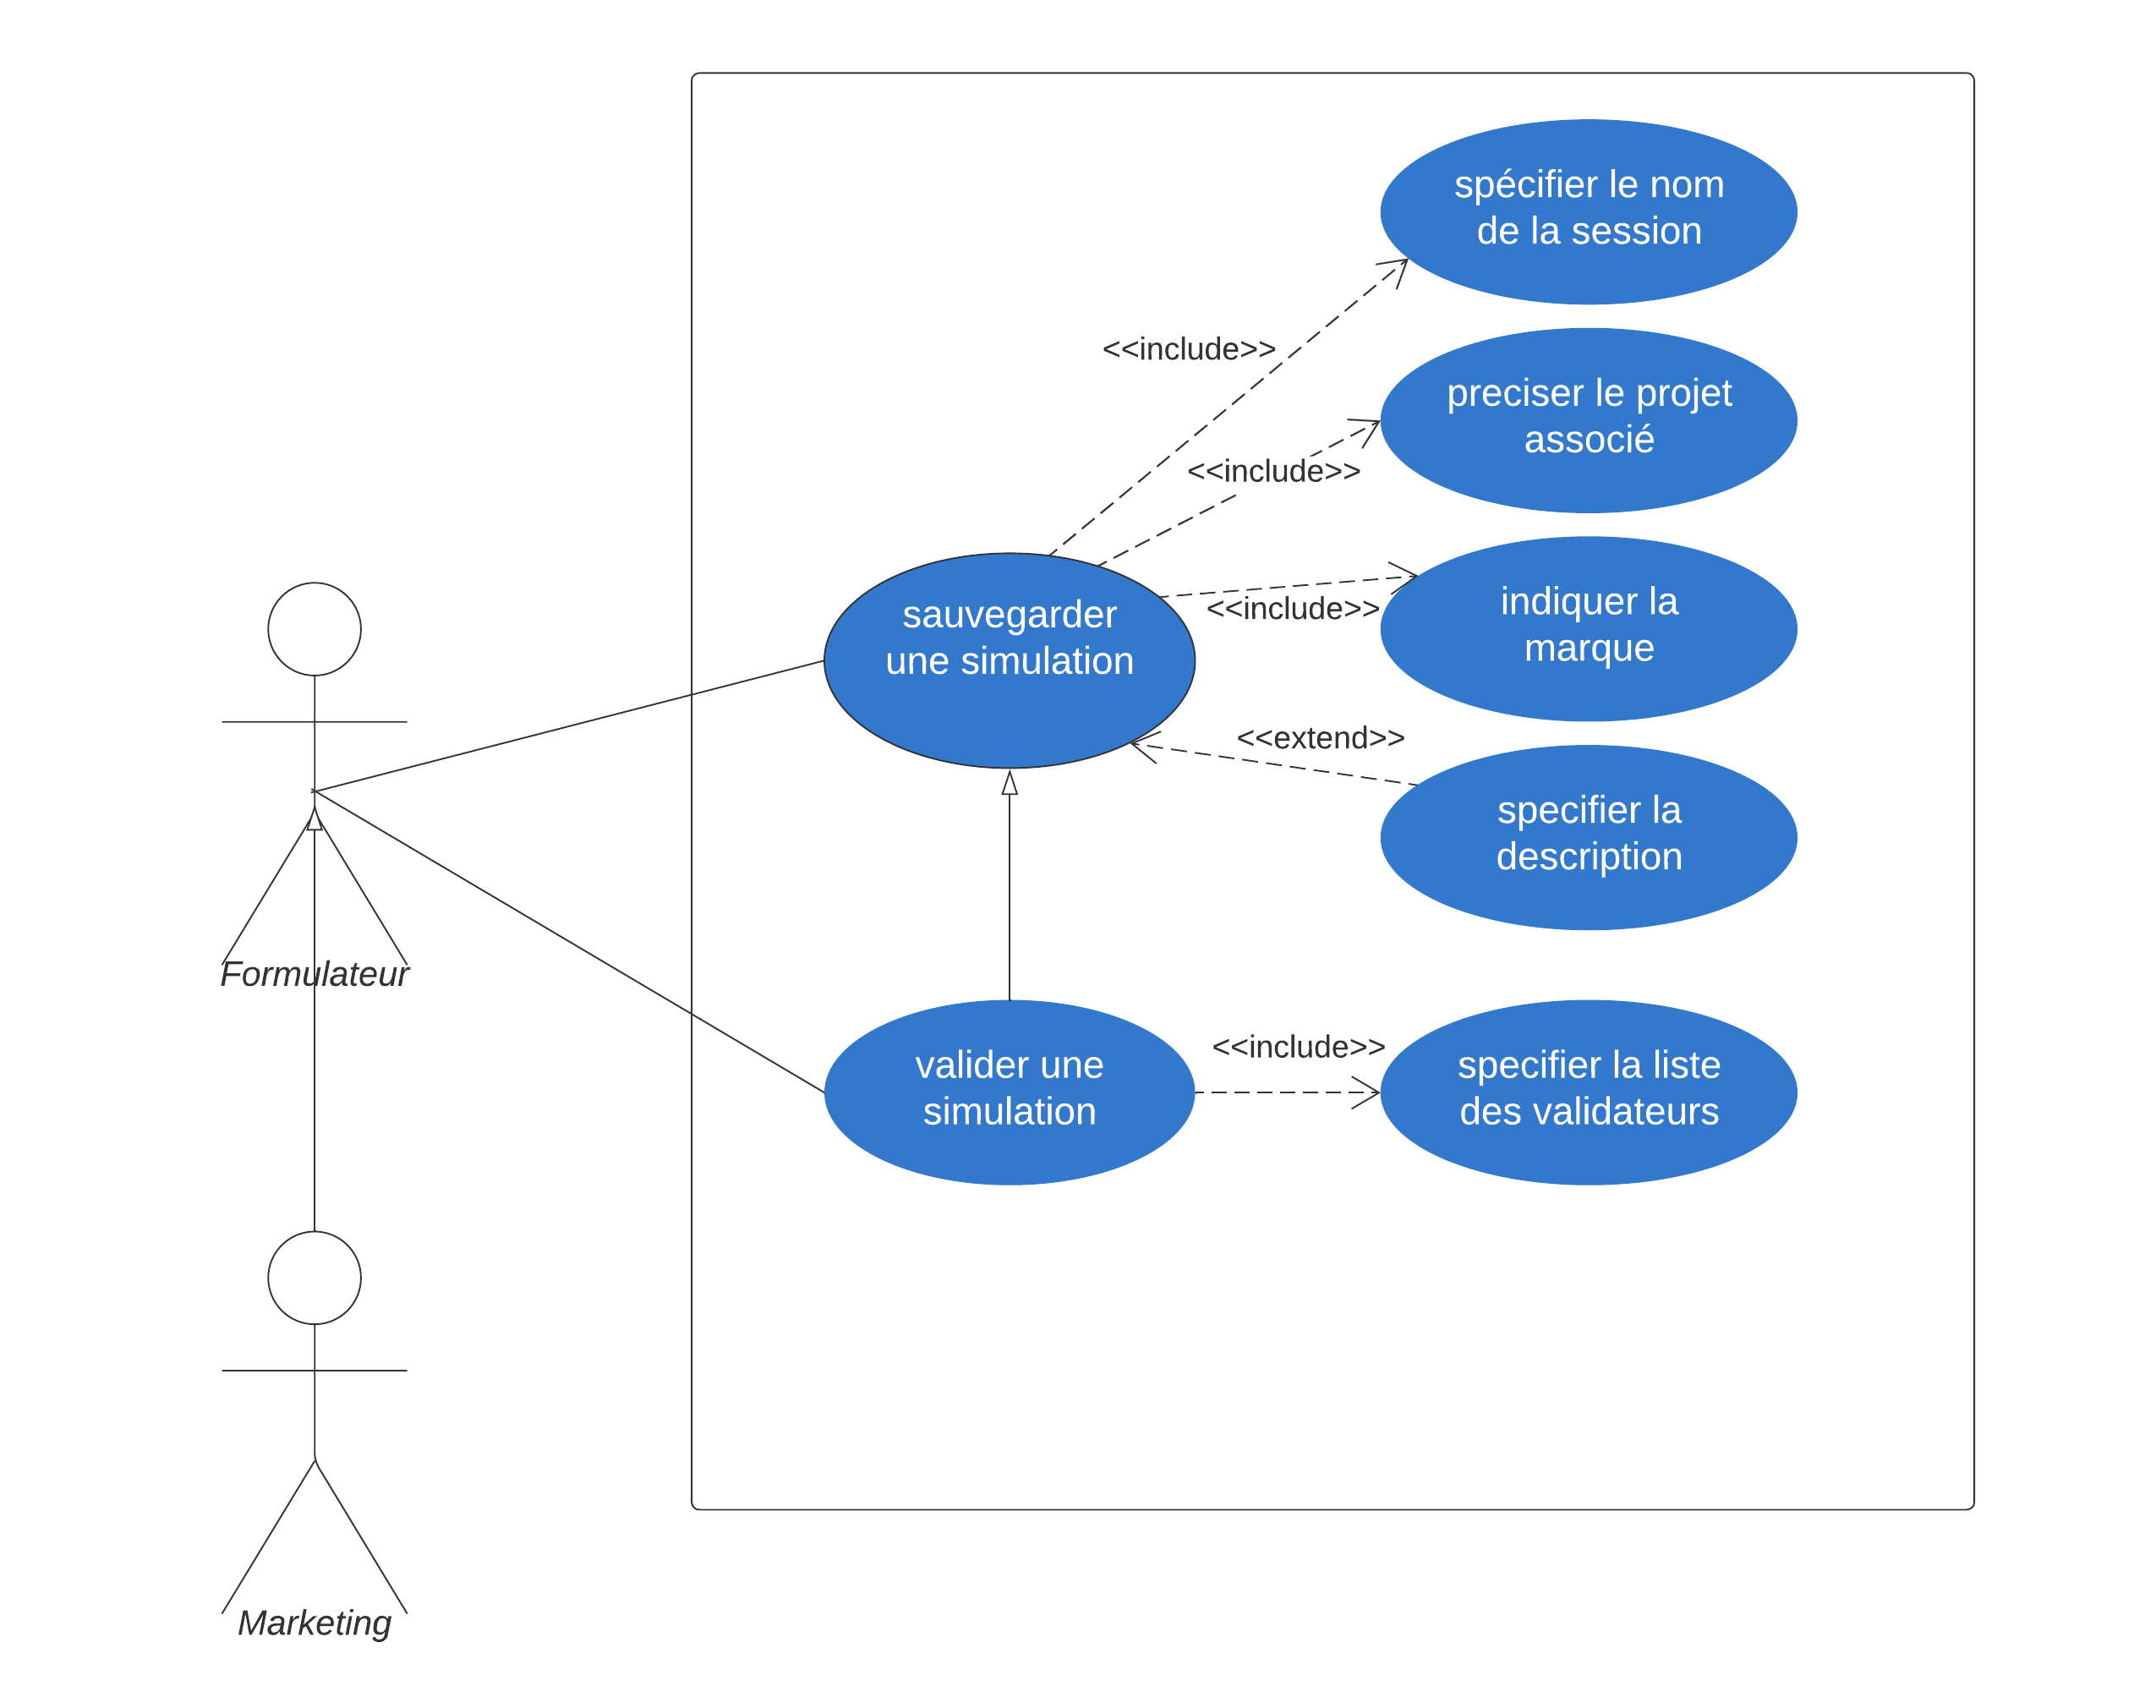
\includegraphics[width=1.1\textwidth,angle=00]{chapitres/chapitre5/figures/Diagramme de cas d'utilisation (sauvegarde).png}
\caption{ Diagramme\textcolor{white}{J}de\textcolor{white}{J}cas\textcolor{white}{J}d’utilisation\textcolor{white}{J}raffiné\textcolor{white}{J}de\textcolor{white}{J}la\textcolor{white}{J} sauvegarde et la validation des simulations. }
\label{fig:diagCase5}
\end{figure}

Apres avoir simuler une couleur de cheveux,le formulateur peut sauvegarder la session en specifiant le titre,la marque,le projet associé et une description.
Le marketteur peut valider une simulation en specifiant la liste des validateurs.

\newpage
La\textcolor{white}{J}figure \ref{fig:diagCaseRaf5} \textcolor{white}{J}illustre\textcolor{white}{J}le\textcolor{white}{J}diagramme\textcolor{white}{J}de\textcolor{white}{J}cas\textcolor{white}{J}d’utilisation\textcolor{white}{J}raffiné\textcolor{white}{J}de\textcolor{white}{J}la simulation d'une nouvelle couleur de cheveux.
\begin{figure}[!ht]\centering
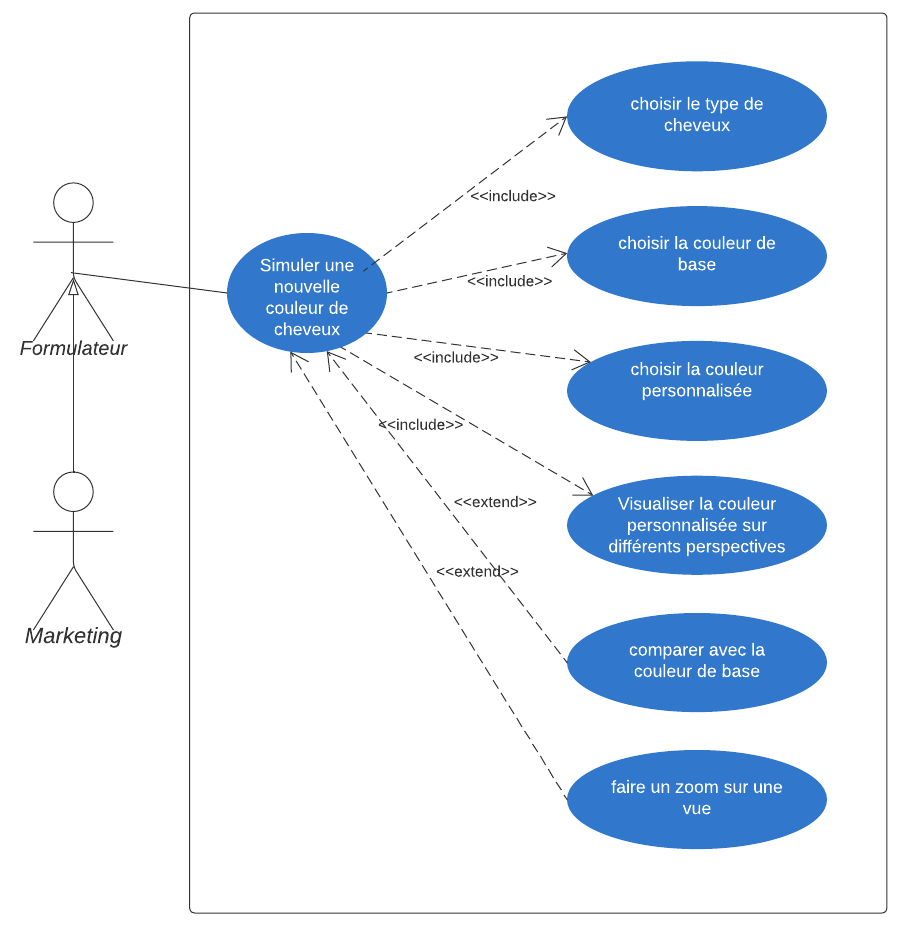
\includegraphics[angle=00]{chapitres/chapitre5/figures/Diagramme de cas d'utilisation (simulation).png}
\caption{ Diagramme de cas d’utilisation raffiné de la simulation d'une nouvelle couleur de cheveux }
\label{fig:diagCaseRaf5}
\end{figure}

Apres avoir specifier le type des cheveux,la couleur de base et la couleur personnalisée et en cliquant sur le boutton simuler,
Pour simuler une nouvelle couleur de cheveux,l'utilisateur doit specifier le type des cheveux,la couleur de base et la couleur personnalisée.En cliquant sur le boutton simuler,l'utilisateur aura les images synthétisées en differentes vues.Ensuite,l'utilisateur peut comparer la couleur de base avec la couleur personnalisée ou effectuer un zoom sur une vue.


\newpage
\newpage
\subsection{Maquette\textcolor{white}{J}de\textcolor{white}{J}l’interface\textcolor{white}{J}de création d’une simulation}
\begin{figure}[!ht]\centering
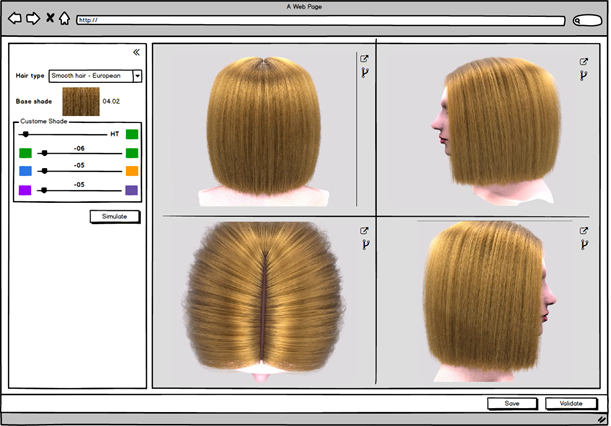
\includegraphics[width=0.7\textwidth,angle=00]{chapitres/chapitre5/figures/Maq-1.png}
\caption{Maquette\textcolor{white}{J}de\textcolor{white}{J}l’interface\textcolor{white}{J}de création d’une simulation}
\label{fig:OffreSeq}
\end{figure}

\subsection{Maquette\textcolor{white}{J}de\textcolor{white}{J}l’interface\textcolor{white}{J}de sauvegarde des simulations}
\begin{figure}[!ht]\centering
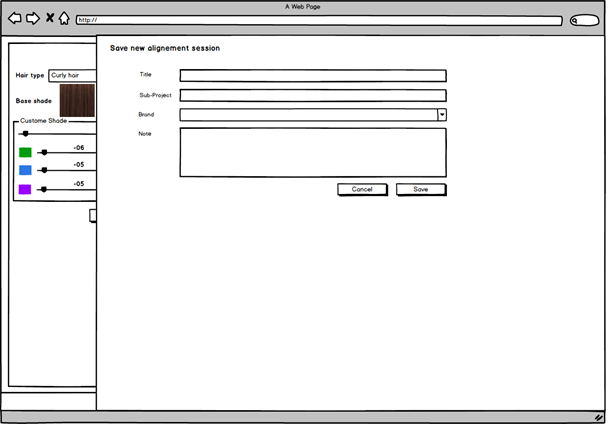
\includegraphics[width=0.7\textwidth,angle=00]{chapitres/chapitre5/figures/Maq-2.png}
\caption{Maquette\textcolor{white}{J}de\textcolor{white}{J}l’interface de sauvegarde des simulations}
\label{fig:OffreSeq}
\end{figure}

\newpage
\subsection{Maquette\textcolor{white}{J}de\textcolor{white}{J}l’interface de visualisation des simulations}
\begin{figure}[!ht]\centering
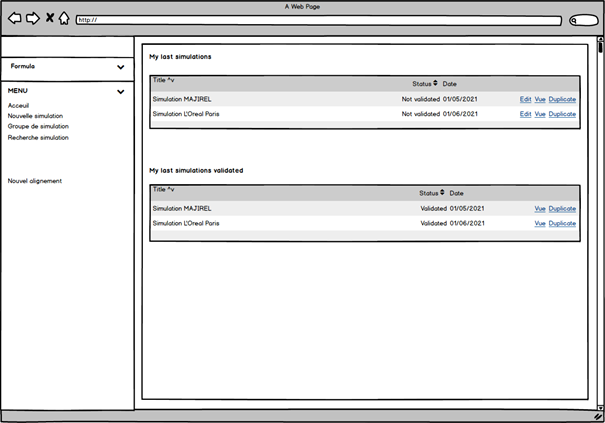
\includegraphics[width=0.7\textwidth,angle=00]{chapitres/chapitre5/figures/Maq-3.png}
\caption{Maquette\textcolor{white}{J}de\textcolor{white}{J}l’interface de visualisation des simulations}
\label{fig:OffreSeq}
\end{figure}

\newpage
\section{Conception}
\subsection{Diagramme\textcolor{white}{J}d'activité\textcolor{white}{J}du\textcolor{white}{J}processus\textcolor{white}{J}de\textcolor{white}{J}création\textcolor{white}{J}de simulation}
 
\begin{figure}[!ht]\centering
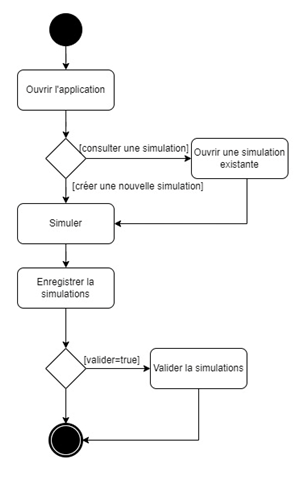
\includegraphics[width=0.6\textwidth,angle=00]{chapitres/chapitre5/figures/ActChap5.png}
\caption{Diagramme\textcolor{white}{J}d'activité\textcolor{white}{J}du\textcolor{white}{J}processus\textcolor{white}{J}de\textcolor{white}{J}création de simulation}
\label{fig:OffreAct}
\end{figure}

Lorsque l'utilisateur ouvre l'aaplication,il peut ouvrir une simulation existante ou creer une nouvelle simulation puis simuler une nouvelle couleur de cheveux.
Si le marketteur choisi de valider la simulation,il doit specifier la liste des validateurs.

\newpage
\subsection{Diagramme\textcolor{white}{J}de\textcolor{white}{J}séquence\textcolor{white}{J}objet}
\begin{figure}[!ht]\centering
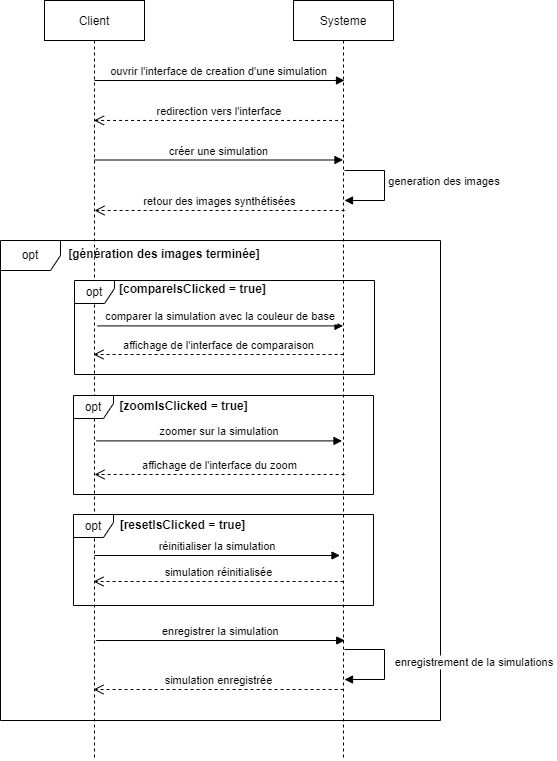
\includegraphics[width=0.8\textwidth,angle=00]{chapitres/chapitre5/figures/Seq.png}
\caption{Diagramme de séquence objet}
\label{fig:OffreSeq}
\end{figure}

Apres avoir preciser les parametres de la simulation,le systeme va proceder la generation des images synthétisées puis les retourner au client.
le client aura un boutton de comparaison ,zoom et reinitialisation.
Si le boutton comparer est cliqué,l'interface de comparaison est affichée. 
Si le boutton zoom est cliqué,l'interface de zoom est affichée pour effectuer un zoom sur les differentes vues . 
Si le boutton reset est cliqué,la simulation est reinitialisée. 

\newpage
\section{Réalisation}
\subsection{Technologies}
\subsubsection*{Reactjs.NET[14]}
ReactJS.NET facilite l'utilisation de React et JSX à partir de C# et d'autres langages .NET, en se concentrant spécifiquement sur ASP.NET MVC. Il prend en charge à la fois ASP.NET 4 (avec MVC 4 ou 5) et ASP.NET Core MVC.


\subsubsection*{Webpack[15]}
Webpack est un outil logiciel open-source de type « module bundler », conçu pour faciliter le développement et la gestion de sites et d'applications web modernes.
Ce logiciel permet de réaliser un certain nombre de tâches fastidieuses et répétitives liées au développement comme la compilation du code source et le déploiement d'applications sur des serveurs de manière automatique


\subsubsection*{D3.js [16]}
D3.js est une bibliothèque graphique JavaScript qui permet l'affichage de données numériques sous une forme graphique et dynamique. Il s'agit d'un outil important pour la conformation aux normes W3C qui utilise les technologies courantes SVG, JavaScript et CSS pour la visualisation de données.


\newpage
\subsection{Développement de la pipette de couleur LAB}
Pour générer des images synthétisées, le moteur graphique a besoin principalement de la couleur de la teinte dans l’espace chromatique L*A*B* qui est l'espace le plus utilisé dans les contrôles colorimétriques modernes. Ce mode est idéal pour mesurer des colorants ou des pigments. 
Les paramètres du système L*a*b* sont :
La clarté L* qui prend des valeurs entre 0 (noir) à 100 (la luminance de la surface) ;
Le paramètre a* représente la valeur sur un axe vert → rouge qui des prend des valeurs entre -128 et 127.
Le paramètre b* représente la valeur sur un axe bleu → jaune qui des prend des valeurs entre -128 et 127.

\begin{figure}[!ht]\centering
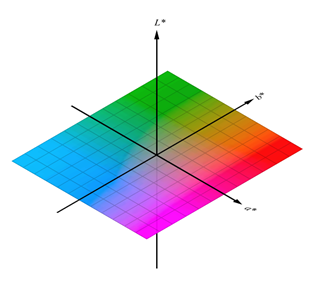
\includegraphics[width=0.5\textwidth]{chapitres/chapitre5/figures/RGB.png}
\caption{Représentation de l'espace L*a*b*}
\label{fig:git}
\end{figure}

\newpage
L’objectif était de développer la pipette de couleur du système LAB et une section pour visualiser la couleur résultante de la combinaison des valeurs LAB en convertissant la couleur LAB en RGB et Hexadécimal 
La figure \ref{fig:pip} représente le prototype de la pipette LAB

\begin{figure}[!ht]\centering
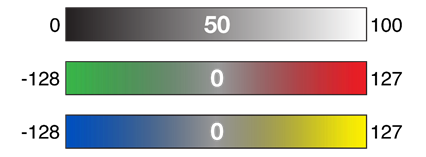
\includegraphics[width=0.3\textwidth]{chapitres/chapitre5/figures/RGB-2.png}
\caption{Le prototype de la pipette LAB}
\label{fig:pip}
\end{figure}

Pour développer cette pipette, on a utilisé la bibliothèque d3-color pour pouvoir utiliser les algorithmes de la colorisation LAB et D3.js qui va permettre la visualisation de données de notre spectre. Chaque paramètre doit avoir une glissière pour choisir la valeur et un fond pour visualiser le spectre.
La figure \ref{fig:rgb} représente notre pipette dans l’état initial et dans l’état de changement des paramètres.
\begin{figure}[!ht]\centering
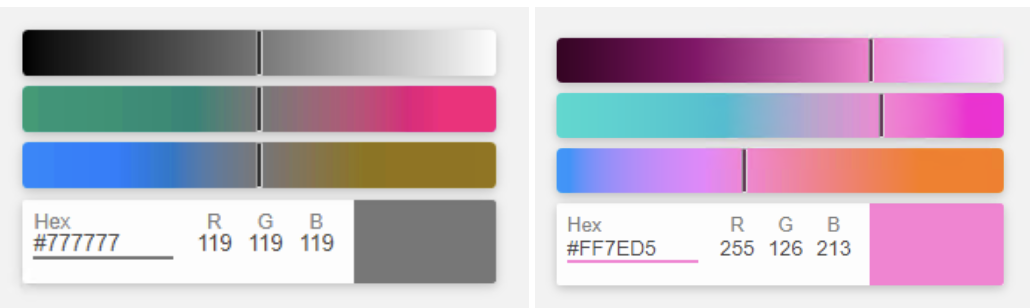
\includegraphics[width=0.6\textwidth]{chapitres/chapitre5/figures/RGB-Double.png}
\caption{L’état initial et dans l’état de changement des paramètres.}
\label{fig:rgb}
\end{figure}

\subsection{La communication la partie frontend et backend}
Pour envoyer des requêtes HTTP au serveur « backend », on a créé notre propre client http en utilisant la dépendance de Microsoft « Autorest ». En se basant sur le fichier « swagger.json » qui contient tous les informations sur notre API, on va exécuter un script PowerShell permettant la génération d’un dossier intitulé « /api » contenant une instance qui va nous permettre de communiquer avec le serveur. Ce script doit être exécuté avec PowerShell ISE.
La figure \ref{fig:dossier} suivante présente le dossier généré.
\begin{figure}[!ht]\centering
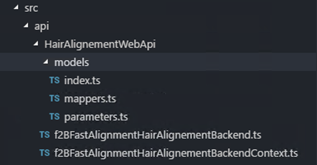
\includegraphics[width=0.4\textwidth]{chapitres/chapitre5/figures/TS.png}
\caption{Le\textcolor{white}{J}dossier\textcolor{white}{J}généré}
\label{fig:dossier}
\end{figure}

\newpage
\subsection{La gestion des simulations}
\textbf{Consulter les simulations}
\\
Les utilisateurs peuvent visualiser la liste des simulations ainsi que rechercher une simulation ou filtrer la liste par état.

La figure \ref{fig:simu} représente la consultation des simulations
\begin{figure}[!ht]\centering
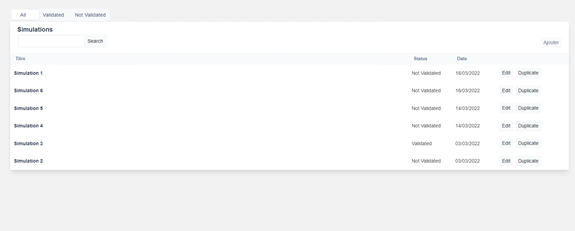
\includegraphics[width=0.8\textwidth]{chapitres/chapitre5/figures/ListSimu.png}
\caption{List des simulations}
\label{fig:simu}
\end{figure}

\textbf{Création d’une simulation}
\\
La figure \ref{fig:simu2} illustre l’interface graphique de la création d’une simulation.
\begin{figure}[!ht]\centering
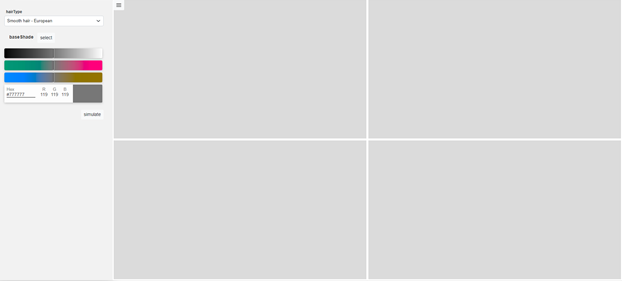
\includegraphics[width=0.8\textwidth]{chapitres/chapitre5/figures/AjoutSimu.png}
\caption{L’interface graphique de la création d’une simulation}
\label{fig:simu2}
\end{figure}

\textbf{La communication en temps réel}
\\
La récupération des images synthétisées se fait en temps réel pour cela on a développé le client SignalR avec la dépendance @microsoft/signalr
La première étape de la communication est de demander un identifiant de connexion du serveur backend puis exécuter une requête http GET au serveur backend sous l’url « /alignement/Get » tout en spécifiant l’identifiant de la connexion avec le bus signalR. Puis le serveur backend va publier les images synthétisées au client en utilisant cet identifiant. 
Ensuite, les images seront placées sur l’écran comme indiqué dans la figure ci-dessous 
\begin{figure}[!ht]\centering
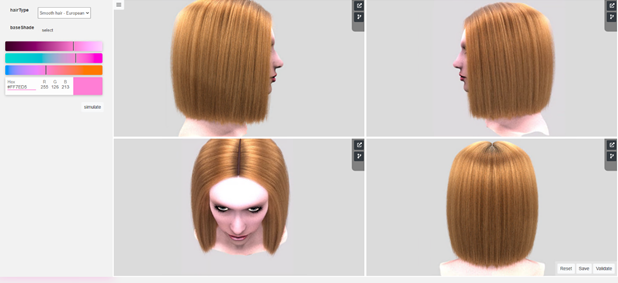
\includegraphics[width=0.8\textwidth]{chapitres/chapitre5/figures/EditSimu.png}
\caption{L’interface graphique de la création d’une simulation}
\label{fig:git}
\end{figure}

Les boutons Reset, Save et Validate seront affichés dès que toutes les vues seront disponibles. Le serveur « backend » va continuer d’envoyer des images de qualité supérieure. Ces derniers vont remplacer les anciennes images instantanément pour pouvoir remarquer la différence.

\textbf{La modification d’une simulation}
\\ 
La figure \ref{fig:simuModif} illustre l’interface graphique de la modification d’une simulation
\begin{figure}[!ht]\centering
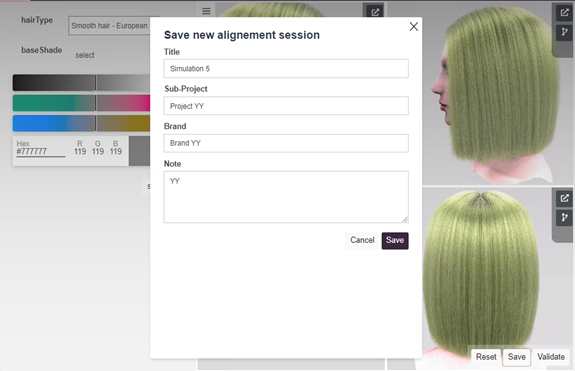
\includegraphics[width=0.8\textwidth]{chapitres/chapitre5/figures/NewAlignment.png}
\caption{L’interface graphique de la modification d’une simulation}
\label{fig:simuModif}
\end{figure}

\newpage
\textbf{La comparaison des simulations :}
\\ 
L’utilisateur a la possibilité de comparer entre la couleur de la teinte généré et la couleur de base en appuyant sur le bouton « compare » qui affichera l’interface de comparaison indiqué dans la figure \ref{fig:comp} ci-dessous
\begin{figure}[!ht]\centering
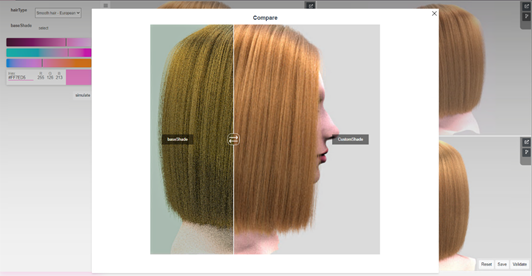
\includegraphics[width=0.7\textwidth]{chapitres/chapitre5/figures/Compare.png}
\caption{L’interface de comparaison}
\label{fig:comp}
\end{figure}

\textbf{Ajuster automatiquement la taille de l’écran}
\\
Notre solution va être utilisée dans des ordinateurs, des tablettes, ou même des écrans géants donc c’est très important d’offrir une expérience confortable sur des écrans de tailles très différentes.
La figure \ref{fig:auto} ci-dessous présente notre application sur les dimensions d’une tablette
\begin{figure}[!ht]\centering
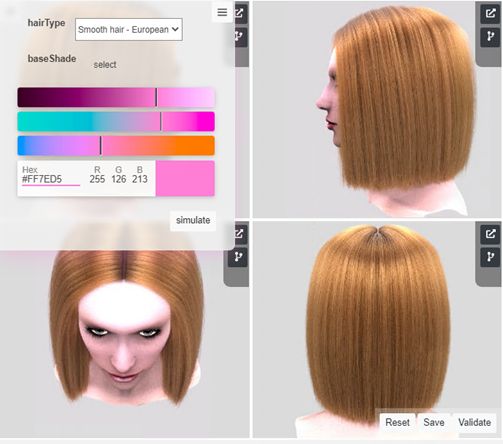
\includegraphics[width=0.6\textwidth]{chapitres/chapitre5/figures/Responsive.png}
\caption{Les dimensions d’une tablette}
\label{fig:auto}
\end{figure}

\newpage
\textbf{Intégration de la solution dans la Formulation Center}
\\
La Formulation Center est la nouvelle plateforme qui rassemble des informations entre plusieurs plateformes et référentiels. Cette plateforme est au service de plus de 5 000 collaborateurs travaillant à la Recherche & Innovation et dans les Divisions de L’Oréal. La plateforme serve de façon transverse différents métiers et fonctions : formulateurs, chimistes, directeurs scientifiques, achats, développement opérationnel, etc.
Les solutions du Formulation Center sont développées en .NET Core MVC. Pour cela, on doit faire le packaging de notre application avec Webpack le système de regroupement de modules populaire puis intégrer le module dans un projet .NET Core en utilisant la dépendance ReactJS.NET qui va faciliter l’interaction de React avec .NET Core.
Ensuite on a intégré le projet « RDLoreal.FormulationCenter » et « RDLoreal.GUI » dans notre solution 
La figure \ref{fig:dox} ci-dessous présente l’arborescence de la solution après l’intégration des projets du Formulation center 

\begin{figure}[!ht]\centering
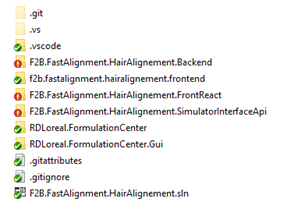
\includegraphics[width=0.6\textwidth]{chapitres/chapitre5/figures/Structure.png}
\caption{L’arborescence de la solution après l’intégration des projets du Formulation center }
\label{fig:dox}
\end{figure}

Avec l’intégration de la Formulation Center, on a la possibilité d’utiliser les services implémentés par le département Recherche et développement. 
Pour la récupération de l’utilisateur connecté on a exploiter l’interface « IHttpContextAccessor » du projet « RDLoreal.GUI » dans notre solution en injectant la dépendance dans notre Controller. 
La figure \ref{fig:arbo} ci-dessous présente l’application avec l’intégration du Formulation Center

\begin{figure}[!ht]\centering
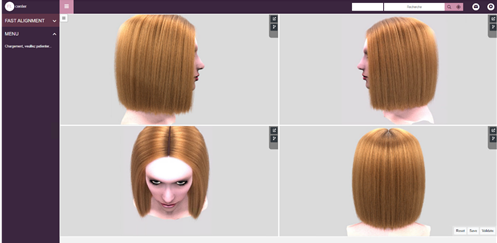
\includegraphics[width=0.8\textwidth]{chapitres/chapitre5/figures/IntegrationFC.png}
\caption{L’arborescence de la solution après l’intégration des projets du Formulation center }
\label{fig:arbo}
\end{figure}

\newpage
\textbf{Le déploiement de la plateforme}
\\
Sur le serveur IIS, on a créé un dossier pour contenir les fichiers et dossiers publiés de l’application. Le chemin de ce dossier est fourni à IIS en tant que chemin d’accès physique à l’application. Puis, On a publié notre solution en choisissant l’option de publication Dossier. Notre solution était prête dans le répertoire « bin/Release/netcoreapp/publish ». Ensuite, on a déplacé le dossier de publication vers le serveur physique « FRRDAPP423D » où vous devez déployer et on a configuré IIS dans le serveur. Après, l’équipe de déploiement a attribué le nom de domaine suivant a notre application « https://dev-formulationcenterfildomain.rd.loreal »



\section*{Conclusion}
Au cours de ce chapitre, nous avons réussi à développer la partie partie frontend et l'integrer dans la plateforme « Formulation Center » et enfin deployer la solution.
